%!TEX root = ../memoire.tex

\chapter{Génération automatique de texte}

%%%%%%%%%%%%%%%%%%%%%%%%%%%%%%%%%%%%%%%%%%%%%%%%%%%%%%%
% --------- I N T R O   ---------
%%%%%%%%%%%%%%%%%%%%%%%%%%%%%%%%%%%%%%%%%%%%%%%%%%%%%%%

La \acf{GAT} est une branche du \acf{TAL} à la croisée des chemins entre l'intelligence artificielle et la linguistique computationnelle \citep{ReiterBuildingNaturalLanguage2000}. L'objectif de la \ac{GAT} est de produire du texte compréhensible en langue naturelle à partir de données (non-linguistiques). Bien que cet objectif soit commun à tous les générateurs de texte, il existe diverses méthodes pour y arriver. La diversité des méthodes est une conséquence directe de la combinaison des divers types d'inputs possibles et des multiples approches de réalisation. Effectivement, les systèmes de \ac{GAT} peuvent prendre en input du texte, des données numériques et même des images \citep{thomason:coling14}. \draft{De plus, \cite{gatt18} notent qu'il y a un affaissement des frontières (systèmes hybrides) entre les méthodes traditionnelles de réalisation (à base de patrons, à base de règles, stochastiques).}\FL{ça va plus loin}

Les premiers systèmes de \ac{GAT} ont été conçus pour générer des rapports automatiquement afin de faciliter le travail humain \citep{ReiterBuildingNaturalLanguage2000}. Effectivement, \cite{DaoustJSREALTextRealizer2015} expliquent que la \ac{GAT} nous permet de générer un résumé d'information compréhensible pour un humain, tandis que la lecture des données brutes lui seraient indéchiffrables. Ces tâches automatisées permettent d'éviter des coûts en termes de ressources et de temps. Autrement, la production de tels rapport est faite par un humain, ce qui entraîne des coûts importants souvent prohibitifs.

Les textes générés automatiquement n'ont pas besoin d'être lus par une grande quantité de gens pour être considérés utiles. Dès qu'ils remplissent leur fonction auprès d'une poignée de gens, leur raison d'être est justifiée. Ces textes produits automatiquement peuvent aussi être extrêmement adaptés à leur public puisque les systèmes de \ac{GAT} peuvent générer du texte en fonction du lecteur. Effectivement, quelques systèmes de \ac{GAT} ont intégré l'aspect utilisateur à leur génération de texte. Il est donc possible de générer un rapport en fonction du niveau de compréhension des données d'un utilisateur donné. Par exemple, un professionnel, un technicien ou un client \citep{1948c0b7a8ca42679cad977bb2cdddc2} se verraient offrir des rapport différents.
\FL{ce paragraphe est redondant, tu dis trois fois la même chose}

D'autres chercheurs ont aussi poussé la \ac{GAT} vers le domaine journalistique. Il y avait une forme de demande pour cette branche qu'est le robo-journalisme. Un contexte propice à ce genre de système est le manque de couverture médiatique d'un match sportif. Graĉe au robo-journalisme, on peut générer un résumé d'un match à partir des données brutes de celui-ci. Par exemple, on peut savoir: qui a compté, à quelle minute, les fautes, etc. \citep{W17-3513}.
\FL{lisser}

Il est aussi important de préciser que la \ac{GAT} présente une valeur linguistique théorique. En effet, les linguistes s'en servent pour tester leurs théories et vérifier si leur modélisation de la langue contient des erreurs \citep{DanlosPresentationmodelegeneration1983}. 

Dans le cadre de ce mémoire, nous élaborerons plus précisément sur une partie du processus de la \ac{GAT}: la réalisation. Cependant, avant de décrire cette étape, nous allons jeter les bases de la \ac{GAT} en décrivant le pipeline classique.
\FL{ce paragraphe va plus loin}

%%%%%%%%%%%%%%%%%%%%%%%%%%%%%%%%%%%%%%%%%%%%%%%%%%%%%%%
% --------- P I P E L I N E   ---------
%%%%%%%%%%%%%%%%%%%%%%%%%%%%%%%%%%%%%%%%%%%%%%%%%%%%%%%

\section{Pipeline classique GAT} \label{ppc}

Selon \cite{ReiterBuildingNaturalLanguage2000}, un système de \ac{GAT} se découpe en six modules, que nous illustrons à la figure~\ref{fig:Pipeline}.\FL{enlève INPUT et OUTPUT dans la figure} De façon plus grossière, on peut séparer ces modules en deux étapes majeures: le \emph{quoi-dire} et le \emph{comment-le-dire} \citep{DanlosPresentationmodelegeneration1983}, qui correspondent aux \emph{early process} et \emph{late process} de \cite{gatt18}. Le \emph{quoi-dire} fait référence à la sélection du contenu, la structuration du document et l'agrégation. Puis le \emph{comment-le-dire} fait référence à toutes les étapes subséquentes:\FL{mets jamais d'espace avant un signe de ponctuation, laisse \LaTeX\ gérer ça} la lexicalisation, la génération d'expressions référentielles et la réalisation linguistique. Pour mieux comprendre ce processus séquentiel, nous décrirons en quelques lignes chacune des étapes qui le compose.

\begin{figure}[htb] % utilise toujours [htb]
	\centering
	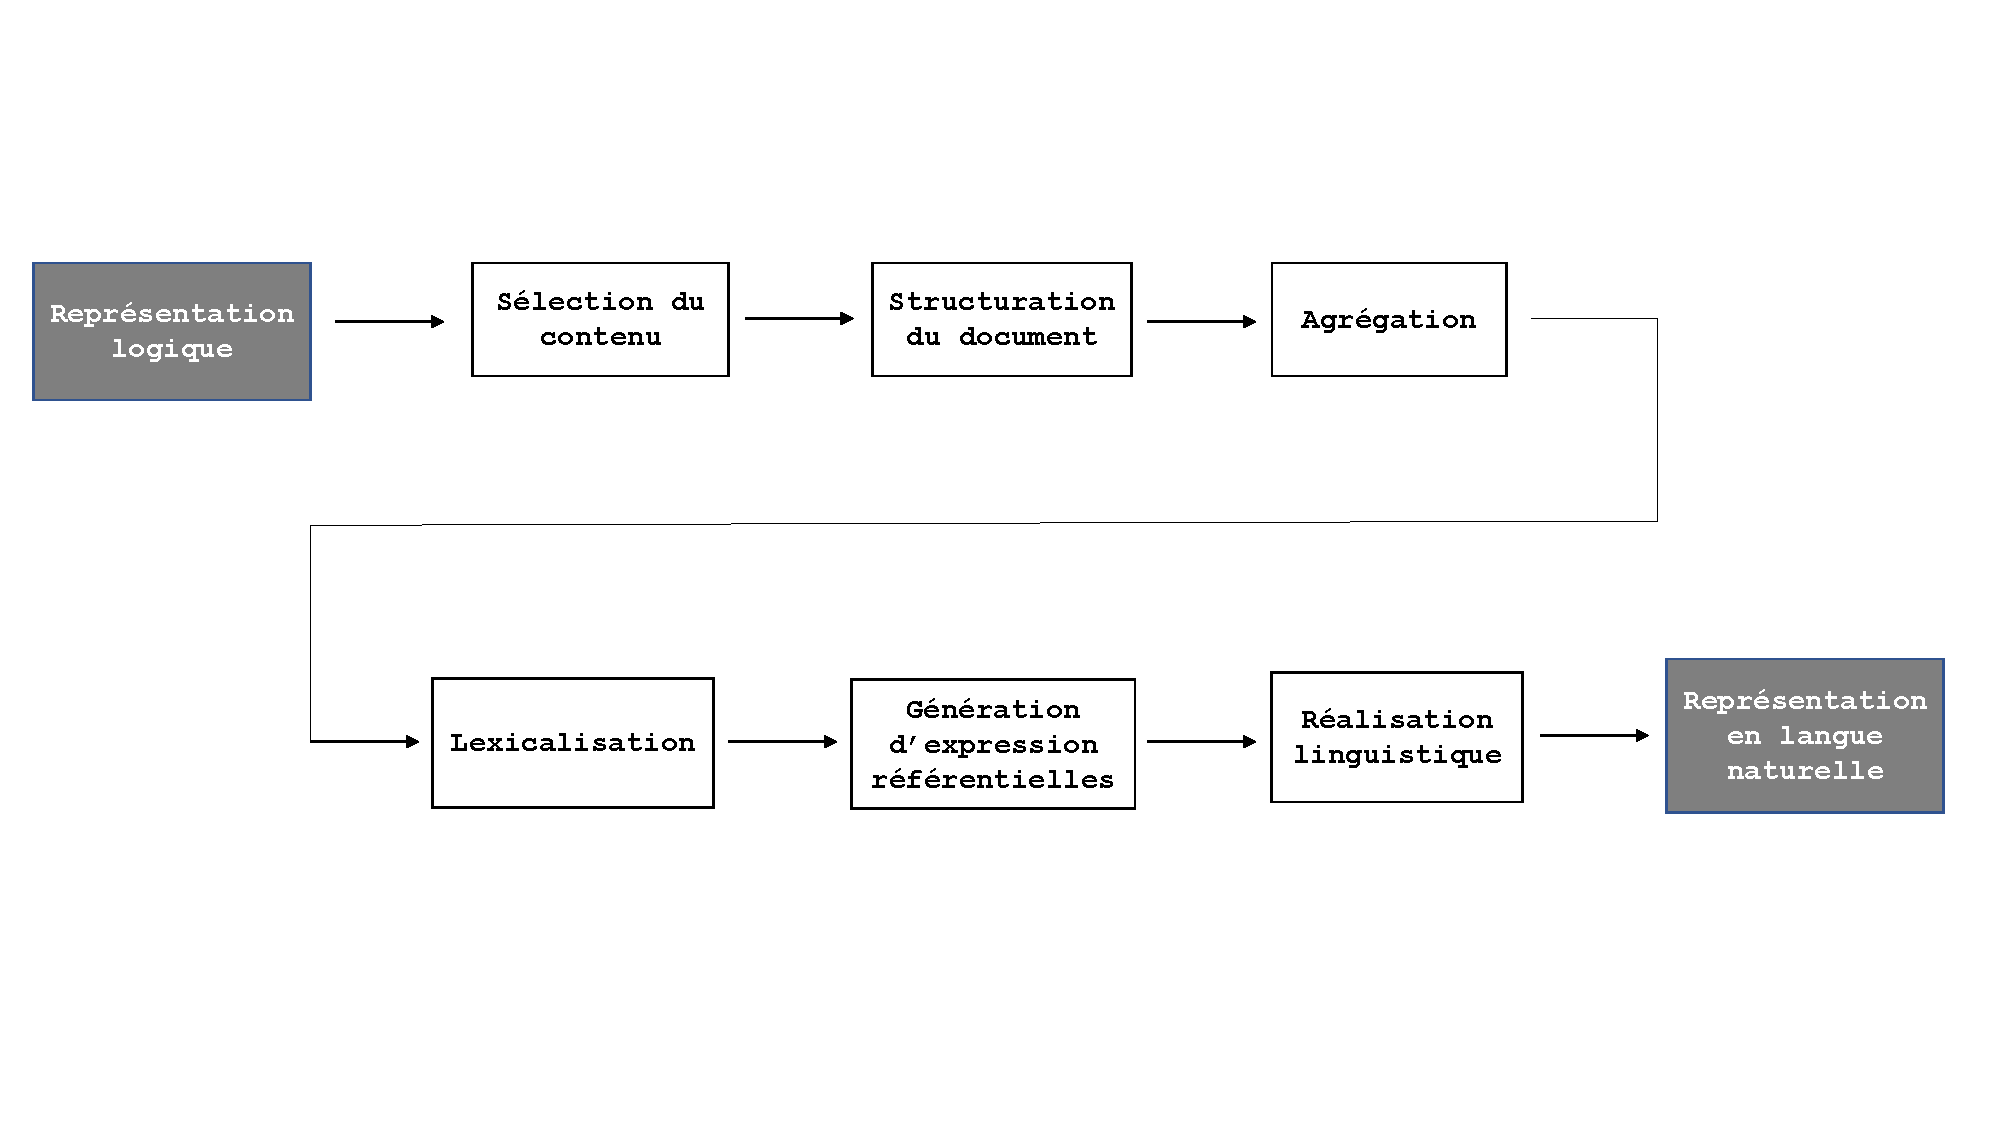
\includegraphics[width=1\textwidth, trim = {0cm 0cm 0cm 0cm},clip]{ch2/figs/pipeline.pdf}
	\caption{Pipeline classique}
	\label{fig:Pipeline}
\end{figure}

\FL{ça vaut pas la peine de faire des sous-sections numérotées pour des petits paragraphes comme ça. commence chaque paragraphe par le nom de l'étape que tu décris, comme ça on voit clairement la structure. tu peux même les mettre en gras pour faciliter la lecture}

Un système de \ac{GAT} doit départir les informations qui seront dans le texte de celles qui n'y seront pas. Il s'agit donc de déterminer ce qui est pertinent dans les données brutes. Par exemple, si on souhaite générer le compte rendu d'un match de soccer, on ne voudrait probablement pas mentionner toutes les passes et toutes les fautes commises durant ce match, même si ces informations figurent dans les données de base. La sélection du contenu dépend aussi beaucoup du public à qui le texte est adressé et de l'objectif du texte: on ne présente pas la même information à un expert et à un novice. Dans le cas d'un compte rendu sportif, par exemple, on pourrait vouloir adapter le texte en fonction de l'équipe préférée du lecteur.

Après avoir sélectionné le contenu, un système de \ac{GAT} doit créer le plan du texte. Il s'agit de décider dans quel ordre présenter les informations sélectionnées. Cette étape est une représentation ordonnée et structurée du message à transmettre. Reprenons l'exemple du soccer. En fonctions des données choisies, le texte devra débuter par les informations générales liées au match (où et quand le match s'est déroulé), suivi du nom des équipes qui s'opposaient, de qui a gagné, puis des faits saillants du match.

L'agrégation est l'étape où on combine des messages en une seule phrase afin de rendre le texte plus fluide et agréable à lire. Les messages sélectionnés dans le plan (structuration du document) n'ont pas à être exprimé dans des phrases individuelles si on est capable de les combiner \citep{ChengCapturingInteractionAggregation2000}. Bref, cette étape sert à éviter la redondance et un style trop télégraphique.

À l'étape de la lexicalisation, on commence à traduire les données non-linguistiques en langue naturelle. Cette partie est très importante car on y sélectionne les mots qui seront utilisés pour transmettre le message. Comme il existe naturellement plusieurs manières de rendre une même idée en mots, cette tâche peut devenir assez complexe si on veut que le système tienne compte des subtilités de la langue. La sélection des mots peut ainsi se faire à divers niveaux d'abstraction. Un niveau plus abstrait requière plus de travail et est plus complexe à mettre en place, mais génère plus de possiblités au moment de la réalisation. \cite{ElhadadFloatingConstraintsLexical1997} prônaient une approche en faveur de la lexicalisation profonde.\FL{exemple soccer}

La génération d'expressions référentielles est très similaire à la lexicalisation car on choisit comment se réaliseront certaines entités. Le but est de s'assurer que le lecteur puisse distinguer correctement chaque entité. Pour cela, il faut trouver la meilleure façon de référer à une entité. Pour ces raisons, on l'appelle souvent \scare{l'étape discriminatoire}.\FL{exemple soccer pour parler d'un même joueur: le (position), la jeune recrue, Joe McCain, McCain, Little-Joe, le récipiendaire du prix McKenna, etc.}

\label{real}
La dernière étape est la réalisation linguistique. Lorsque tous les mots et les expressions référentielles ont été choisis, on peut réaliser le texte final. Cette tâche implique l'application de traits morpho-syntaxiques aux lexèmes et la linéarisation des structures. Elle inclut aussi l'insertion des mots fonctionnels (auxiliaires, déterminants,etc.) et la ponctuation. \draft{question pour françois: est-ce que le passage de concept/sémantique à la syntaxe se fait en même temps que la lexicalisation dans ces systèmes ?}\FL{dur à dire, c'est souvent broche-à-foin, et on peut dire en simplifiant que la lexicalisation, c'est ça leur étape de Sém-Synt}

L'étape de la réalisation linguistique nous intéresse particulièrement, donc nous allons élaborer sur celle-ci.

\subsubsection{À base de patrons}
\FL{ces sous-sections devraient aller dans la prochaine section. crée une sous-section Types d'approches, et sous celle-ci décrit ces approches (peut-être pas nécessaire d'avoir une subsubsection?)}
Cette approche est souvent utilisée pour générer du texte dans des domaines spécifiques comme la météo ou les sports. Dans ces contextes, la variation linguistique est réduite au minimum puisque chaque réalisation de texte se fait à partir d'un moule fixe \citep{mcroy_channarukul_ali_2003}. Les phrases en \ref{template} provenant de l'article de \cite{gatt18} démontrent comment les patrons s'utilisent.

\ex. \label{template}
	\a.\$player scored for \$team in the \$minute minute. 
	\b. Ivan Rakitic scored for Barcelona in the 4th minute.

En \ref{template}, le patron contient trois variables, marquées par les \$. Celles-ci peuvent être respectivement comblées par un nom de joueur, suivi d'un nom d'équipe et d'une indication temporelle. L'avantage de cette approche est qu'on peut prévoir exactement ce qui sera généré, ce qui diminue les risques d'erreurs. L'inconvénient est qu'ils sont très rigides. Cependant, les réalisateurs à base de patrons peuvent être complémentés par des règles de grammaire, ce qui les rend plus flexibles. Toutefois, puisqu'ils sont codés à la main, ces sytèmes ont l'inconvénient d'être coûteux à développer. Ils peuvent aussi être combinés à de l'apprentissage machine pour automatiser l'écriture des patrons, qui rend la tâche moins coûteuse \citep{gatt18}.

\subsubsection{À base de règles grammaticales}
Les modèles à base de règles grammaticales s'emploient autant dans les domaines spécifiques (météo, sport, etc.) que les domaines généraux (conversation libre). Ils se prêtent bien à la langue courante puisqu'ils sont conçus pour être très flexibles. Dans ces systèmes, la combinaison de règles de grammaire et de dictionnaires mène à la bonne formation de phrases. Cependant, les grammaires et dictionnaires sont codés manuellement, ce qui demande du temps et des ressources.

\subsubsection{Méthodes statistiques}
Il existe divers emplois des méthodes statistiques. On peut les utiliser pour filtrer les sorties d'un système. Dans ce contexte, un modèle probabiliste déterminera quelle sortie est la meilleure candidate \citep{LangkildeForestbasedStatisticalSentence2000}. On appelle cela l'approche \emph{generate-and-filter}. On peut aussi développer un modèle probabiliste pour apprendre automatiquement la correspondance entre les inputs et les textes voulus,  par apprentissage automatique sur de large corpus \citep{WhiteMinimalDependencyLength2012}. Cela diminue considérablement la charge de travail manuelle.

\subsubsection{Approches à base de règles versus approches statistiques}

\FL{pas la même chose que l'autre paragraphe en haut?}

Traditionnellement, les systèmes de \ac{GAT} tendaient vers des systèmes encodés manuellement. Mais, de tels systèmes nécessitaient du temps et des ressources. Cela a poussé plusieurs chercheurs à automatiser la réalisation linguistique \citep{LangkildeForestbasedStatisticalSentence2000}. L'avantage immédiat de tels systèmes est leur demande plus faible en termes de temps et de ressources. 

\cite{BelzSystemBuildingCost2009} se sont\FL{attention au texte qui entoure les citations: si t'as Belz et Kow (2009), alors le sujet est pluriel, donc "se sont"} demandé si le temps qu'on gagnait en automatisant la réalisation se faisait au détriment de la qualité, et si c'était le cas, à quel point. L'évaluation s'est faite en utilisant un système à base de règles, puis un système statistique pour effectuer la même tâche de réalisation. L'évaluation se faisait en deux temps. D'abord une évaluation humaine pour traiter la qualité des textes des deux systèmes, puis une évaluation métrique faite automatiquement. Suite à l'analyse de l'évaluation, ils nous démontrent que les évaluations humaines pointaient en faveur des systèmes à base de règles. De plus, ils concluaient que certaines évaluations métriques surévaluaient parfois les systèmes statistiques et sous-évaluaient les systèmes manuels.

D'ailleurs, de son côté, Reiter s'est aussi penché sur la question et a fait un survol du sujet dans son blog.\footnote{\draft{\url{http://...}, date}} Selon lui, même si les systèmes d'apprentissage automatique génèrent de bons textes la plupart du temps, ils génèrent occasionnellement des textes bizarres et inappropriés. Il souligne aussi que les évaluations des systèmes statistiques sont souvent basées sur la moyenne des textes générés correctement. Cela ne rend pas compte de l'ampleur de certaines erreurs. Ce comportement n'est pas approprié dans des domaines professionnels ou personnels où des utilisateurs comptent sur la qualité des textes, entre autre, car ils prendront potentiellement des décisions en fonction de leur lecture. De plus, Reiter ajoute que lorsque des incongruités sont générées, les systèmes basés sur des méthodes statistiques ont plus de difficulté à les corriger. En revanche, les systèmes à base de règles permettent de cerner les problème avec plus de facilité et de les corriger en rectifiant la règle problématique directement. Cependant, Reiter termine son blog en soulignant que la \ac{GAT} a beaucoup à gagner avec les méthodes statistiques. Il suggère de se servir de celles-ci pour automatiser des parties du processus de réalisation à base de règles.

%%%%%%%%%%%%%%%%%%%%%%%%%%%%%%%%%%%%%%%%%%%%%%%%%%%%%%%
% --------- R É A L I S A T I O N   ---------
%%%%%%%%%%%%%%%%%%%%%%%%%%%%%%%%%%%%%%%%%%%%%%%%%%%%%%%


\section{Réalisation}

Puisque nous avons maintenant traité du processus global de \ac{GAT} et des différentes méthodes de réalisation, nous pouvons entrer dans les détails de la tâche qu'est la réalisation linguistique, dans laquelle s'insère notre travail.

Tel qu'explicité à la figure~\ref{fig:Pipeline}, la réalisation est la dernière étape dans le processus de \ac{GAT}. Toutefois, pour beaucoup de chercheurs, elle ne représente pas uniquement les tâches décrites précédemment. Il règne en effet un certain flou autour de ce qui constitue la réalisation. Pour certains, elle correspond exactement à ce qu'on a présenté dans la section \ref{real}. On appellera cela la réalisation de surface, puisque la réalisation se fait à partir d'un input beaucoup plus près du texte (des structures syntaxiques lexicalisées). Pour d'autres, la réalisation se fait à partir de données plus abstraites, en amont de la lexicalisation. Ce type de réalisation plus profonde prend généralement en input des structures pré-syntaxiques. On les appellera des réalisateurs profonds. Dans ces systèmes, les informations lexicales et grammaticales seront encodées dans des dictionnaires et des grammaires plus complexes permettant de traiter l'interface sémantique-syntaxe. Finalement, ces systèmes profonds sont généralement liés à une théorie linguistique leur permettant de modéliser le langage et de l'encoder dans un système informatique.

%%%%%%%%%%%%%%%%%%%%%%%%%%%%%%%%%%%%%%%%%%%%%%%%%%%%%%%
% --------- R É A L I S A T E U R   S U R F A C E ---
%%%%%%%%%%%%%%%%%%%%%%%%%%%%%%%%%%%%%%%%%%%%%%%%%%%%%%%

\subsection{Réalisateurs de surface}

Dans cette section, nous présenterons trois réalisateurs de surface connus: SimpleNLG, JSreal et RealPro.

\subsubsection{SimpleNLG}
SimpleNLG \citep{GattSimpleNLGRealisationEngine2009} est un réalisateur de surface pour l'anglais écrit en java. Le texte est réalisé à partir d'une structure syntaxique déjà lexicalisée encodée en XML. Par la suite, le réalisateur effectue les opérations morphologiques nécessaires (flexion, dérivation, ajout d'auxiliaires, gestion de l'accord) tout en linéarisant le texte.

Puisqu'il s'agit d'un réalisateur à base de règles, SimpleNLG est doté d'une grammaire et d'un dictionnaire. Ce dernier encode les propriétés syntaxiques et morphologiques des unités lexicales. Puis, le module grammatical contient des règles permettant le passage de la syntaxe à la morphologie.

SimpleNLG sépare son processus de réalisation en quatre étapes. Premièrement, les lexèmes compris dans la structure d'input sont mis en correspondance avec leurs entrées de dictionnaire. Deuxièmement, on détermine les traits spécifiques des lexèmes. Troisièmement, on combine les lexèmes en créant des syntagmes de plus en plus larges, jusqu'à ce que l'entièreté de la phrase forme un syntagme phrastique. Finalement, celui-ci est linéarisé\FL{un syntagme, c'est pas déjà linéarisé?} puis les lexèmes sont accordés en fonction des règles morphologiques pour obtenir les formes fléchies.

\draft{mettre les citations dans references.bib}Noter que SimpleNLG a été traduit dans plusieurs langues: espagnol, italien, et français, portugais (Mazzei et al., 2016, Ramos-Soto 2017, Vaudry et Lapalme 2013 ; Oliveira et Sripada).

\draft{utiliser les formats de descriptions de phrase TST}
La figure \ref{simplenlg} permet de réaliser\FL{c'est la figure qui permet ça?} la phrase \form{Refactoring is needed}. Elle provient du GitHub de SimpleNLG.\footnote{\url{https://github.com/simplenlg/simplenlg/blob/master/docs/XMLRepresentationOfTextSpecifications.pdf}}

\begin{lstlisting}[language=Xml, caption=Structure d'input dans SimpleNLG, label=simplenlg]
<Document>
  <child xsi:type="SPhraseSpec">
    <subj xsi:type="VPPhraseSpec" FORM="PRESENT_PARTICIPLE">
      <head cat="VERB">
        <base>refactor</base>
      </head>
    </subj>
    <vp xsi:type="VPPhraseSpec" TENSE="PRESENT" >
      <head cat="VERB">
        <base>be</base>
      </head>
      <compl xsi:type="VPPhraseSpec" FORM="PAST_PARTICIPLE">
        <head cat="VERB">
          <base>need</base>
        </head>
      </compl>
    </vp>
  </child>
</Document>
\end{lstlisting}

\subsubsection{JSreal}
\FL{remplacer par JSRealB: http://rali.iro.umontreal.ca/rali/fr/jsrealb-realisateur-bilingue-de-texte}
JSreal (pour \emph{JavaScript Realiser}) \citep{DaoustJSREALTextRealizer2015} est conçu pour les programmeurs web. Ce réalisateur génère des expressions et phrases bien formées qui peuvent être formattées en HTML pour ensuite être utilisées dans un fureteur. JSreal peut aussi s'employer seul à des fins purement linguistiques. Généralement, les spécificités de JSreal sont assez similaires à celles de SimpleNLG \citep{GattSimpleNLGRealisationEngine2009}.

Pour générer du texte, JSreal prend en input des structures syntaxiques lexicalisées. La construction de la phrase découle de l'application de règles syntaxiques et morphologiques déclenchées par les lexèmes. JSreal fonctionne aussi avec un dictionnaire et une grammaire. Son dictionnaire définit la catégorie des lexèmes qui le peuple et leurs traits lexicaux (genre, nombre, irrégularités, etc.). La grammaire de JSreal contient des règles morpho-syntaxiques qui lui permettent de faire l'accord entre les constituants. Finalement, il existe aussi une version bilingue de JSreal \citep{MolinsJSrealBBilingualText2015} qui incorpore le français et l'anglais.\draft{Présenter la phrase correctement en TST\FL{qu'est-ce que tu veux dire?}}La figure \ref{jsreal} produit la phrase: \form{The cat sat on the coach}. Cet exemple est tiré du GitHub de JSrealB.\footnote{\url{https://github.com/rali-udem/JSrealB}}

\begin{lstlisting}[language=Xml, caption=JSreal, label=jsreal]
JSrealLoader({
        language: "en",
        lexiconUrl: URL.lexicon.en,
        ruleUrl: URL.rule.en,
        featureUrl: URL.feature
    }, function() {
    QUnit.test( "Sentence EN", function( assert ) {
        assert.equal(
            S(
                NP(D("the"), N("cat")),
                VP(V("sit"), PP(P("on"), NP(D("the"), N("coach")))).t("ps")
            )
        
\end{lstlisting}
		
\subsubsection{RealPro}
RealPro \citep{LavoieFastPortableRealizer1997} est implémenté en C++. Il est le plus profond des réalisateurs de surface préséntés ici. Il prend en input des arbres de dépendances, ce qui le distingue des deux autres systèmes discutés plus haut (arbres de constituant) \citep{DaoustJSREALTextRealizer2015,GattSimpleNLGRealisationEngine2009}. L'architecture de RealPro est basée sur la \ac{TST} \citep{melcuk1988}. Brièvement, il s'agit d'une théorie qui divise le langage en quatre niveaux de représentations majeurs: sémantique, syntaxique (profond et de surface), morphologique (profond et de surface), phonologique (profond et de surface) -- ce dernier étant court-circuité pour la génération de texte écrit. Pour plus de détails concernant les arbres de dépendances et la \ac{TST}, voir le chapitre~\ref{chapgendr}.

Le passage de la syntaxe profonde à celle de surface est la première étape pour réaliser du texte dans ce système. Pour ce faire, le logiciel effectue la transition en utilisant un dictionnaire et une grammaire. Les modules dictionnairiques et grammaticaux sont donc réquisitionnés par les diverses composantes du réalisateur au cours de la génération. Le graphique \ref{fig:RealPro} démontre leurs intéractions. \draft{élaborer sur le fonctionnement de RealPro}
\begin{figure}[htb]
	\centering
	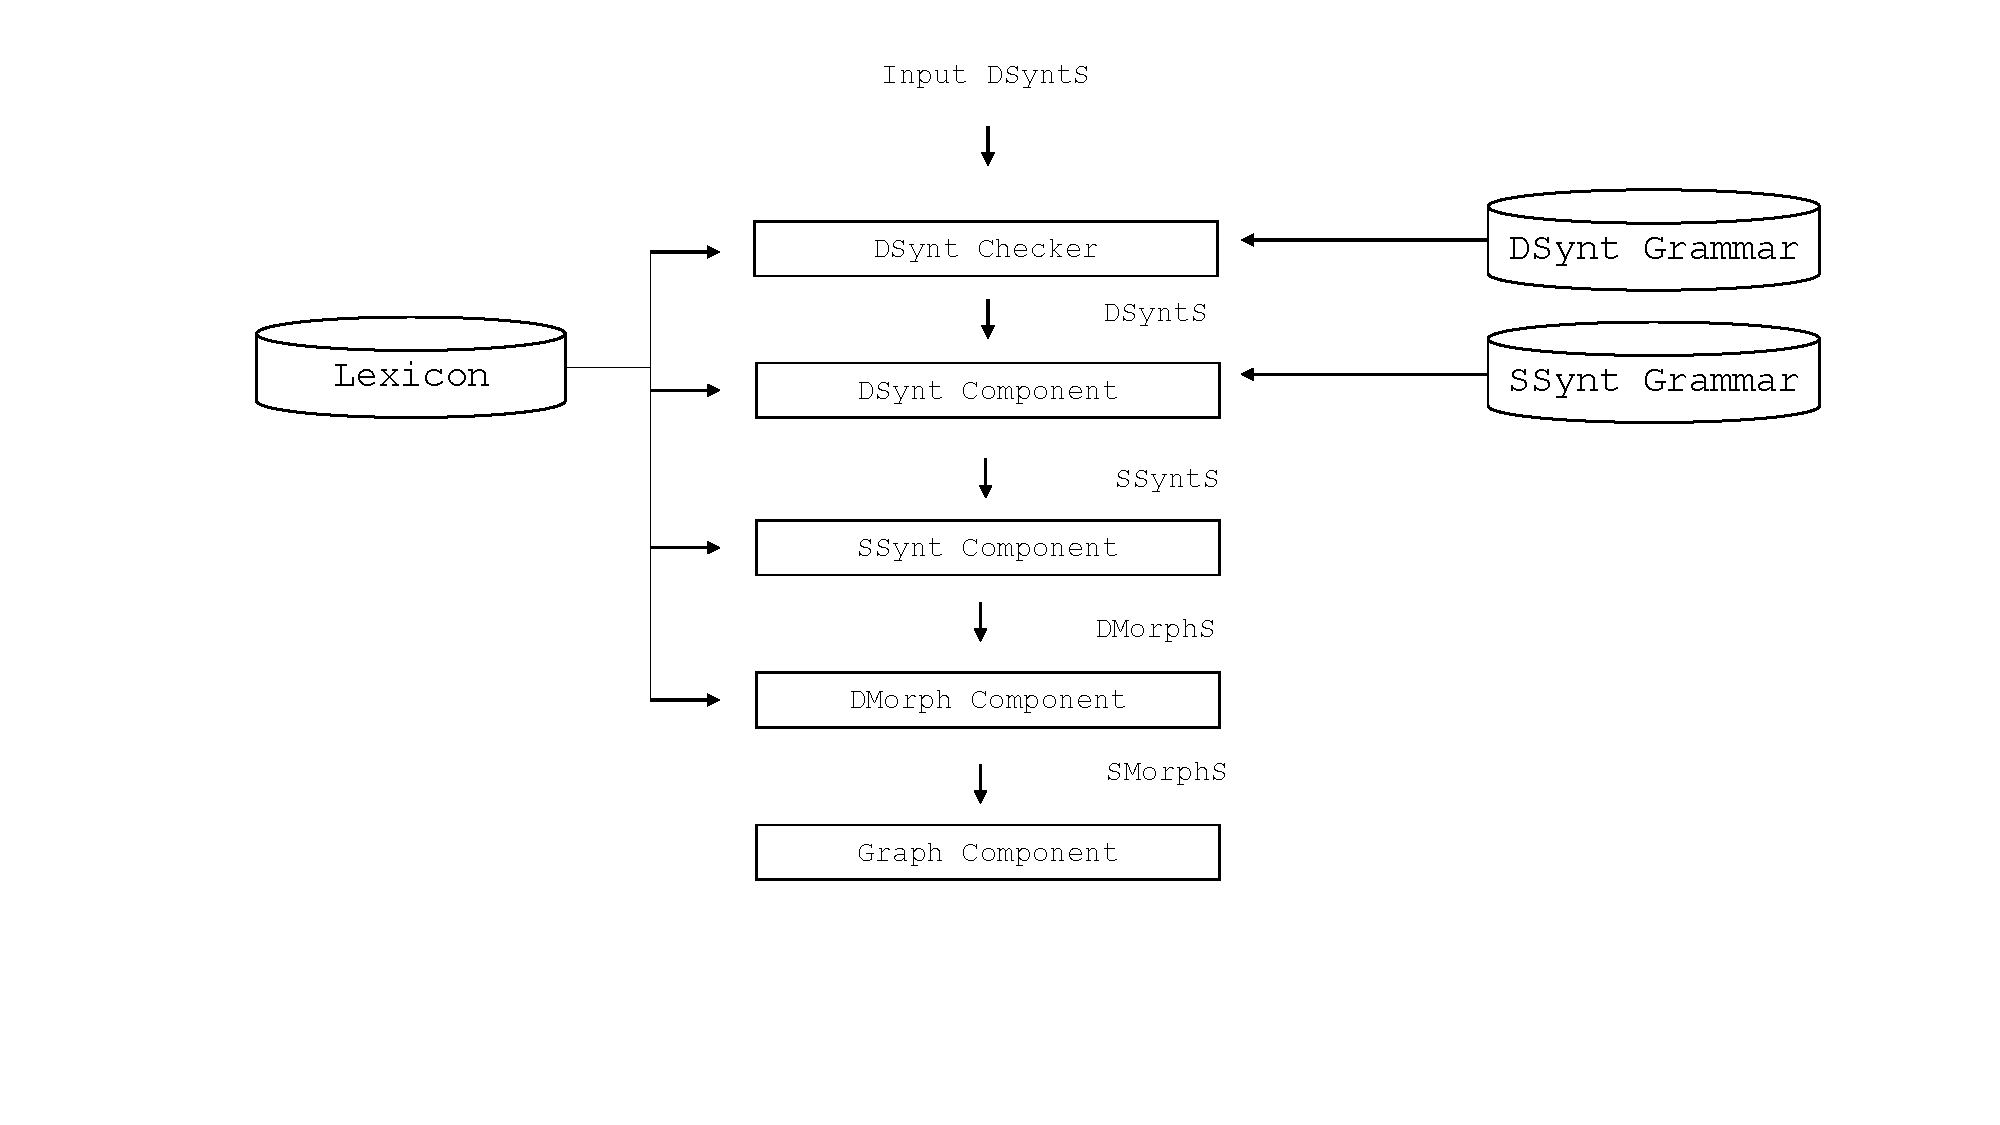
\includegraphics[width=1\textwidth, trim = {0cm 0cm 0cm 0cm},clip]{ch2/figs/realpro.pdf}
	\caption{RealPro}
	\label{fig:RealPro}
\end{figure}

La figure \ref{realpro} est un arbre de dépendance (input) représentant la phrase \draft{changer le format de l'exemple} \form{March had some rain days}.

\begin{lstlisting}[language=Xml, caption=Input, label=realpro]
HAVE1 [tense:past]
(I March [class:proper-noun]
II day [class:common-noun numberpl]
(ATTR rainy [class:adjective]))
\end{lstlisting}

\FL{évite les coupures de page dans un listing, il doit y avoir une option}

%%%%%%%%%%%%%%%%%%%%%%%%%%%%%%%%%%%%%%%%%%%%%%%%%%%%%%%
% --------- R É A L I S A T E U R    P R O F O N D  ---
%%%%%%%%%%%%%%%%%%%%%%%%%%%%%%%%%%%%%%%%%%%%%%%%%%%%%%%

\subsection{Réalisateurs profonds}

Les réalisateurs profonds prennent généralement en input des structures plus abstraites, ce qui entraîne une plus grande flexibilité linguistique dans la réalisation. En effet, les réalisateurs profonds incorporent généralement la lexicalisation, ce qui fait en sorte que les mots à utiliser dans le texte ne sont pas encore fixés \citep{PolguerePourmodelestratifie}. Cela permet de faire usage de paraphrases puisqu'on peut désormais exprimer une même idée de diverses manières. Dans le pipeline classique, comme nous l'avons vu à la section \ref{ppc}, la lexicalisation est opérée avant la réalisation, ce qui fait en sorte que les inputs contiennent déjà des lexèmes et cela restreint grandement les réalisations possibles puisque les lexèmes incorporent des propriétés de combinaitoires bien précises autours desquelles la phrase doit s'articuler. 

Dans cette section, nous présenterons les réalisateurs profonds suivants: KPML, Surge, FORGe et MARQUIS.

\subsubsection{KPML}
KMPL \citep{BatemanEnablingTechnologyMultilingual1997} est un réalisateur multilingue issu du système PENMAN \citep{PenmanOverview}. La théorie linguistique sous-jacente à ce système est la \ac{SFG}\FL{utilise toujours $\backslash ac\{\ldots\}$ et laisse \LaTeX\ gérer s'il faut la forme longue ou courte} \citep{MatthiessenSystemicfunctionalgrammar1997}, qui postule que les choix linguistiques sont déclenchés par l'exécution de fonctions grammaticales. D'un point de vue multilingue, les différentes langues issues de KPML partagent la majorité des fonctions grammaticales. Ces fonctions forment le c\oe{}ur du système, mais il existe aussi quelques fonctions propres à chaque langue pour réaliser les phénomènes linguistiques spécifiques à chacune.

La grammaire de ce système est implémentée à la manière d'un réseau orienté. Chaque intersection dans le réseau correspond à un choix grammatical à faire entre différents traits fonctionnels. Ces choix deviennent de plus en plus précis lorsqu'on avance dans le réseau. Ainsi, la forme de surface d'un input donné est la conséquence du parcours de ces réseaux.

Les informations comprises dans les inputs de ce système sont d'ordre sémantique et syntaxique. Il s'agit de \ac{SPL}.\FL{reformuler} Un \ac{SPL} est une matrice d'attributs et de valeurs. Afin d'illustrer à quoi ressemble l'input, nous présentons la figure \ref{kpml}, qui provient de \cite{ReiterBuildingNaturalLanguage2000} \draft{mettre la phrase dans le bon format: \form{March had some rainy days}.}

\begin{lstlisting}[language=Xml, caption=SPL: input de KPML, label=kpml]
(S1 \ generalized-possession
  :tense past 
	:domain (N1 \ time-interval
	            :lex march
							:determiner zero)
	:range (N2 \ time-interval
	           :number plural
						 :lex day
						 :determiner some
						 :property ascription
						 (A1 \ quality :lex rainy)))
\end{lstlisting}

\subsubsection{Surge}\FL{ça s'écrit d'habitude en majuscules il me semble}
Surge, qui signifie \emph{Systemic Unification Realisation Grammar of English}, est une grammaire de l'anglais \citep{Elhadad98surge:a}. Elle est écrite en \ac{FUF} qui est basé sur \acf{FUG} \citep{KayFunctionalUnificationGrammar1984}. \ac{FUF} est un langage de programmation créé pour construire des grammaires d'unification informatisées.

\ac{FUF} prend en input des \ac{FD}, qui décrivent à la fois le sens d'une phrase et la grammaire.\FL{tu veux dire la structure grammaticale de la phrase, ou vraiment la grammaire de la langue?} Les descriptions fonctionnelles sont aussi des matrices d'attributs et de valeurs. Leur unification fournit les précisions requises pour réaliser l'énoncé. Contrairement aux autres réalisateurs présentés ici, le modèle \ac{FUF} n'utilise pas de dictionnaire car l'information lexicale est encodée directement dans la structure d'input (voir la figure \ref{surge}).

Dans Surge, la réalisation se fait en deux temps. La première étape est de procéder à l'unification des \ac{FD} d'input de la phrase à réaliser. Autrement dit, on enrichit la structure d’input avec les spécifications syntaxiques et morphologiques de la grammaire \ac{FUF}.\FL{pas clair} Ces spécifications indiquent, par exemple, les constructions syntaxiques possibles, l'ordre des mots, comment faire l'accord, etc.

Puis, la deuxième étape est d'effectuer la linéarisation. \ac{FUF} linéarise et applique les traits morphologiques en fonction des spécifications encodées lors de l'unification. L'output est une phrase anglaise exprimant le sens de la \ac{FD} en fonction des contraintes imposées par la grammaire.

Nous reprenons encore un exemple tiré de \cite{ReiterBuildingNaturalLanguage2000} \draft{mettre la phrase dans le bon format: \form{March had some rainy days}.}
\begin{lstlisting}[language=Xml, caption=FD: input de Surge, label=surge]
((cat clause)
 (proc ((type possessive)))
 (tense past)
 (partic ((possessor ((cat proper) head ((lex "March"))))
					(possessed ((cat common) head ((lex day)))
											(describer ((lex rainy)))
											(selective yes) (number plural)))))
\end{lstlisting}

\subsubsection{FORGe}
FORGe est un transducteur de graphes qui génère du texte à l'aide de ressources lexicales dictionnairiques et grammaticales \citep{MilledemoFORGePompeu2017,DBLP:conf/semeval/MilleCBW17}.\FL{cite peut prendre en argument une liste de références, donc tu mets une seule fois la commande} C'est un réalisateur profond qui a hérité de l'architecture de Marquis \citep{WannerMARQUISGENERATIONUSERTAILORED2010}.\FL{ça sera donc logique de présenter MARQUIS en premier} FORGe a été conçu pour l'anglais à la base, mais il se veut multilingue (espagnol, allemand, français et polonais sont en développement). C'est un réalisateur qui peut aisément générer du texte en différentes langues grâce à ses règles grammaticales, qui seront majoritairement partagées par toutes les langues. Les règles fonctionnant pour l'anglais ont ainsi été conçues pour pouvoir fonctionner avec d'autres langues.

La théorie linguistique sous-jacente à ce système est la \ac{TST} \citep{melcuk1988,MelcukSemanticsmeaningtext2012}.\FL{melcuk97,polguere98,kahane06,milicevic06?} D'ailleurs nous verrons plus en détails dans la section \ref{chapgendr} au chapitre suivant comment cette théorie linguistique se prête à des transducteur de graphes.

FORGe prend en input des représentations sémantiques sous forme de graphes orientés acycliques représentant les relations prédicats-arguments entre des sémantèmes (donc, des unités pas encore lexialisées). Pour visualiser de quoi on parle ici, nous vous référons à la structure \#2 dans la figure \ref{fig:marquis} de la section MARQUIS \ref{sectionmarquis}.\FL{donc tu aurais dû présenter MARQUIS en premier} La réalisation de texte dans FORGe se découpe en trois étapes: le transfert de la RSém à la RSyntP, suivi du transfert de la RSyntP à la RSyntS, et finalement de la RSyntS au texte linéarisé et morphologisé. \draft{mettre RSem et cie. au début dans la section Acronyme}\FL{et expliquer au lecteur!}

Le passage de la sémantique à la syntaxe profonde est effectué via un algorithme récursif de type \emph{top-down}. Tel que nous le verrons dans le chapitre suivant à la section \ref{secarbolex}, cet algorithme est aussi appelé l'arborisation. Brièvement, le \emph{top} est la racine de l'arbre de dépendance en développement. Ce top est un noeud vide mais contraint par une partie du discours. On veut que le lexème qui consommera le noeud corresponde à la partie du discours requise par celui-ci. Une fois que le \emph{top} est lexicalisé, on crée de nouvelles branches partant de la racine. Ces branches correspondent aux dépendants du \emph{top}. Ensuite, on crée l'arbre de dépendance en correspondance avec le graphe sémantique d'input. Cette construction se fait sur les bases du dictionnaires et de la grammaire pour que l'arbre final soit la correspondance de l'input et qu'il soit grammatical. Bref, on répète les tâches d'arborisation jusqu'à ce qu'on ait analysé la représentation sémantique au complet.
\FL{reformuler la présentation de top-down; as-tu vérifié que FORGe fonctionne comme ça?}

Ensuite, il faut faire le passage de la syntaxe profonde à la syntaxe de surface. Cela correspond à l'étape où on introduit les mots fonctionnels (prépositions, auxiliaires, déterminants) et les relations de surface (sujet, objet direct, etc.). C'est là que FORGe se démarque de MARQUIS. Ils utilisent un dictionnaire de verbes qui explicitent les comportements des verbes en syntaxe. Cela permet de rendre compte de la richesse linguistique des verbes. Puisque les verbes sont généralement ceux qui contrôlent la structure de la phrase, les dictionnaires de verbes permettent de tenir compte d'un bon nombre de constructions. Nous reviendrons à cette problématique dans la section \ref{problema} au chapitre \ref{chapgendr}.

Finalement, la dernière étape de ce réalisateur consiste à linéariser la structure syntaxique de surface et à appliquer les règles morpho-syntaxiques aux lexèmes pour produire le texte final.

\subsubsection{MARQUIS}\label{sectionmarquis}
Comme FORGe et RealPro, MARQUIS est basé sur la \ac{TST}, mais contrairement aux autres systèmes présentés ici, MARQUIS n'est pas qu'un réalisateur profond. Il s'agit d'un système de \ac{GAT} complet qui effectue toutes les étapes du processus de génération automatique de texte (voir \ref{ppc}). Cependant, nous ne nous intéresserons ici qu'à son module de réalisation profonde.\draft{lareau et wanner 2007} Pour plus d'informations concernant le pipeline complet de MARQUIS, voir \citep{WannerMARQUISGENERATIONUSERTAILORED2010}. 

Le but du projet MARQUIS était de générer, à partir de données brutes, des bulletins météorologiques multilingues sur la qualité de l'air. Ces bulletins sont générés en fonction de l'utilisateur. Autrement dit, ceux-ci se créent des profils avec leurs informations personelles et cela permet à MARQUIS de réaliser du texte en fonction de leur niveau de connaissance du domaine et de leurs besoins de santé. Le tout est fait à partir d'un input conceptuel partagé par toutes les langues traitées par MARQUIS (l'anglais, l'allemand, l'espagnol, le catalan, le portugais, le français, le finnois et le polonais). 

Afin de mieux démontrer le processus de réalisation de MARQUIS et de FORGe (bien que l'input de FORGe commence à la structure \#2). La figure \ref{marquis} suivante représente les diverses étapes entreprises par MARQUIS pour rélaiser du texte.\FL{reformuler}

\begin{figure}[htb]
	\centering
	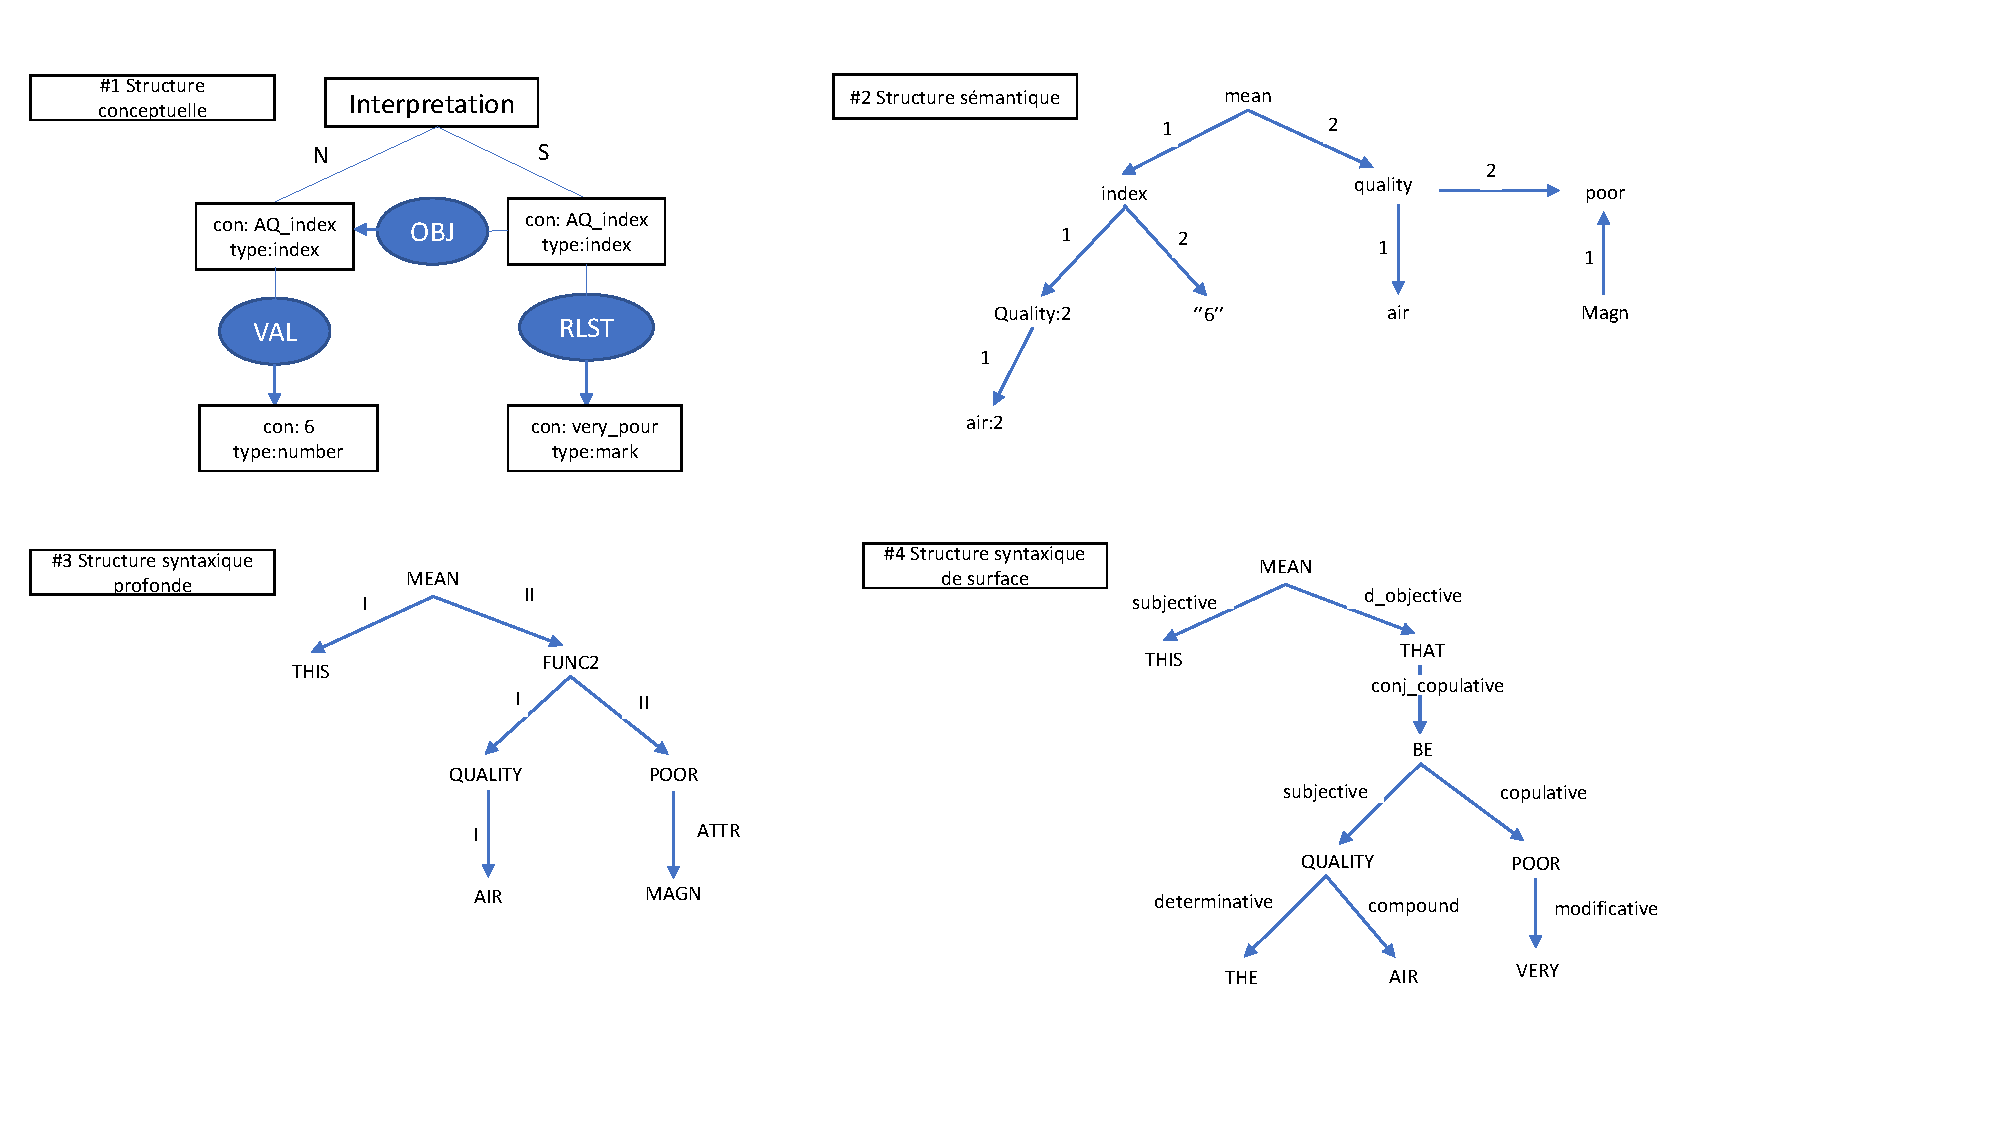
\includegraphics[width=1\textwidth, trim = {0cm 0cm 0cm 0cm},clip]{ch2/figs/marquis.pdf}
	\caption{Pipeline de MARQUIS}
	\label{fig:marquis}
\end{figure}

On voit à la figure \ref{marquis} que MARQUIS prend en input des graphes conceptuels et produit du texte. Entre ces deux niveaux, il y a une série de changements\FL{évite ce mot parce qu'on comprend que tu modifies les structures, ce qui est souvent le mode de fonctionnement des transducteurs de graphes, alors que MATE crée de nouvelles structures} successifs de représentations. Ces changements de représentations sont assurés par: l'information lexicale encodée dans les dictionnaires et les modules de règles qui modélisent chaque interface. 

Nous expliquerons brièvement les mécanismes qui permettent la transition d'une représentation à une autre puisque le tout sera mieux expliquée à la section \ref{secsemsynt}. Alors, il faut d'abord que le système analyse la structure conceptuelle. Ensuite les règles de transduction permettent de passer de la représentation conceptuelle à la représentation sémantique. Le passage des unités conceptuelles aux unités sémantique se fait via l'entremise des dictionnaires respectifs. On a alors une structure sémantique. MARQUIS prendra ce graphe pour en dériver un arbre de dépendances syntaxique profond grâce aux règles de transduction de cette interface. La mise en correspondance d'unités sémantiques et lexicales est opérée grâce au \draft{semanticon et au lexicon} ainsi qu'au dictionnaire de fonctions lexicales. Finalement, les autres transitions de représentations sont assurées par des règles de transductions successives et les informations contenues dans le lexicon. La figure \ref{fig:reglesdict} démontre ces rouages.
\begin{figure}[htb]
	\centering
	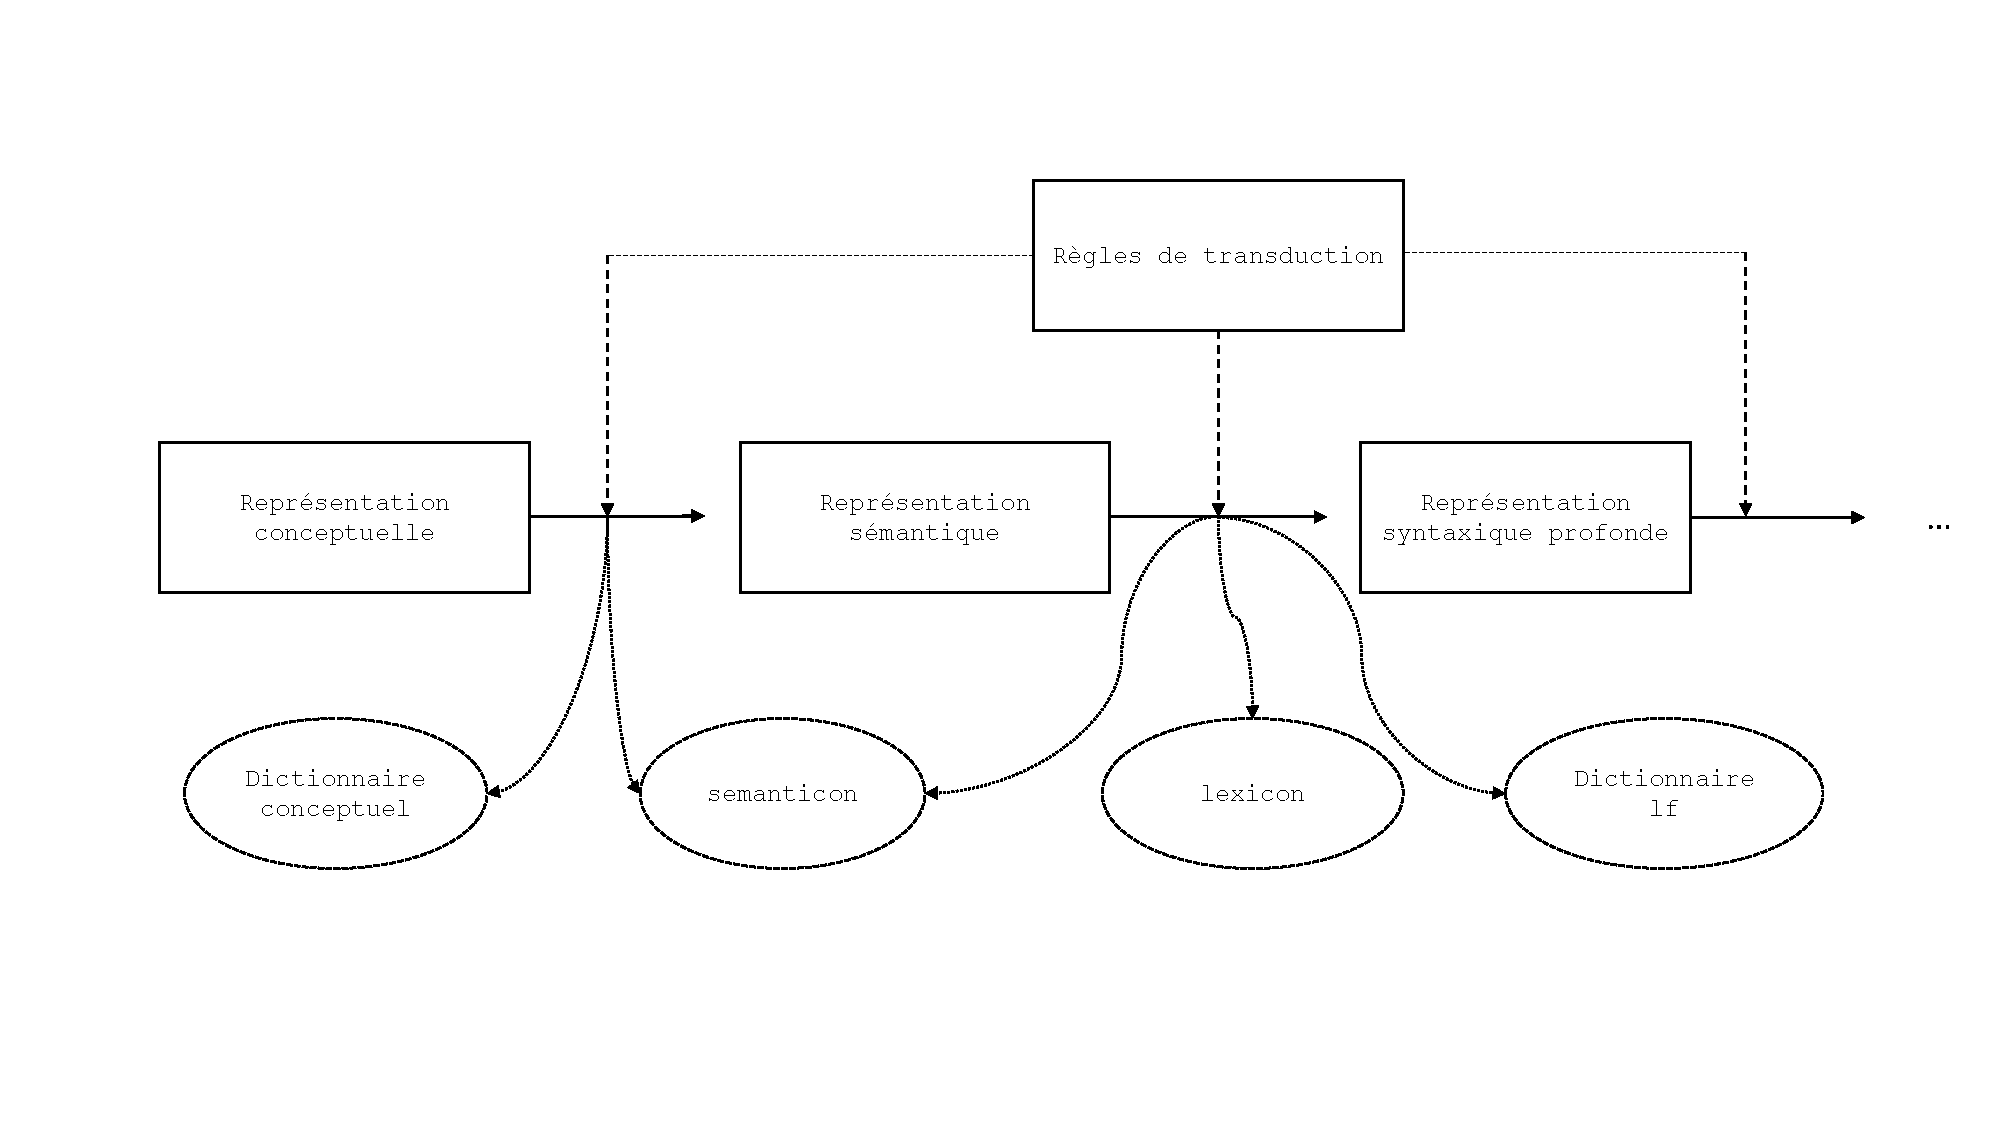
\includegraphics[width=1\textwidth, trim = {0cm 0cm 0cm 0cm},clip]{ch2/figs/module.pdf}
	\caption{Combinaison des règles et dictionnaires}
	\label{fig:reglesdict}
\end{figure}

Pour mieux comprendre à quoi servent les dictionnaires mentionnés dans le paragraphe précédent, nous les décrirons rapidement. Le dictionnaire conceptuel comprend tous les concepts utiles à la génération des rapports sur la qualité de l'air et des termes du domaine général. Ce dictionnaire mappe les concepts aux unités sémantiques pour chaque langue traitée par le système. Le dictionnaire sémantique mappe les unités sémantiques aux lexies. Finalement, il nous faut un dictionnaire lexical qui contient toutes les unités lexicales avec leurs propriétés syntaxiques et morphologiques et leur combinatoire lexicale.

En conclusion, MARQUIS et FORGe partent de niveaux d'abstraction plus profonds que les autres systèmes présentés. Cela leur permet d'être plus flexibles dans leurs réalisations. C'est pourquoi nous utilisons aussi un réalisateur profond très similaire à ces deux réalisateurs. Comme FORGe, nous utiliserons aussi un système basé sur MARQUIS, le système GenDR \citep{lambrey15,LambreyImplementationcollocationspour2017,lareau18}, que le chapitre suivant décrira en détail.